\item Determinar la carga última de una columna de 30 cm x 60cm, compuesta por 4 perfiles ángulos L 3 ½” x 3 ½” x 1/2”.
\begin{itemize}
\item \underline{Datos}
\begin{align*}
& \text{Acero F-24}\\
& E = 200000MPa\\
& f_y = 235MPa\\
& L = 600cm\\
& K_{yz} = 0.7\\
& K_{xz} = 2
\end{align*}
\begin{table}[H]
  \begin{center}
    \begin{tabular}{l|c} % <-- Alignments: 1st column left, 2nd middle, with vertical lines in between
      Perfil & L 3 ½” x 3 ½” x 1/2”\\
      \hline
      $I_x = I_y =$ & $149.65cm^4$ \\
      $r_x = r_y =$ & $2.66cm$ \\
      $r_1 =$ & $1.70cm$ \\
      $e_x = e_y =$ & $2.66cm$ \\
      $A_g =$ & $21.12cm^2$ \\
     
    \end{tabular}
  \end{center}
\end{table}

\begin{figure}[H]
\begin{center}
     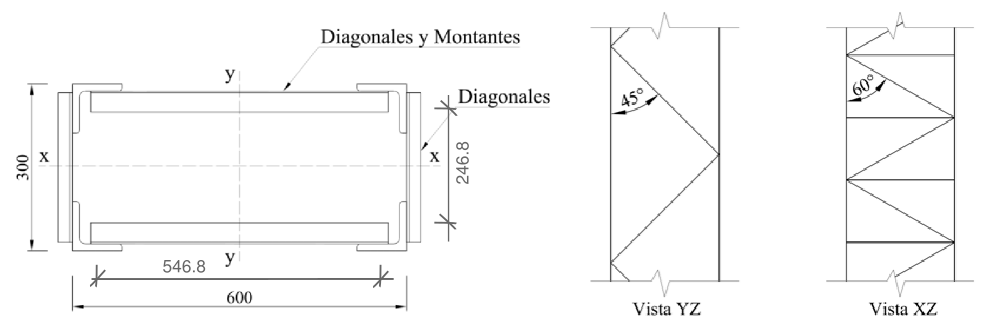
\includegraphics[scale = 1]{chapters/chapter_2/images/figura2_bis.png}
\end{center}
\caption{Columna de 30 cm x 60cm compuesta por perfiles ángulo}
\end{figure}

\newpage
\item \underline{Eje libre x-x $\rightarrow$ Plano YZ}\\
Condición de sustentación empotrado-articulado $\Rightarrow K_{yz} = 0.70$

\item \underline{Momentos de Inercia y Radio de Giro}
\begin{align*}
& d_1 = \frac{Lado_y}{2} - e_y \\
& d_1 = \frac{30cm}{2} - 2.66cm = 12.34cm\\
& I_{xx} = (I_{xx}+A_g \cdot d_1^2) \cdot 4\\
& I_{xx} = (149.65cm^4+21.12cm^2 \cdot (12.34cm)^2) \cdot 4 = \framebox{$13462.84cm^4$}\\
& r_x = \sqrt{\frac{I_{xx}}{A_t}} = \sqrt{\frac{13462.84cm^4}{4\cdot(21.12cm^2)}} = \framebox{$12.62cm$}
\end{align*}

\item \underline{Esbeltez modificada}
\begin{align*}
& \lambda_0 = \frac{K_{yz} \cdot L}{r_x} = \frac{0.70 \cdot 600cm}{2.66cm} = \framebox{$33.27$}\\
& \lambda_0 < 200 \\
& 33.27 < 200 \quad \surd \quad \text{Verifica} \\
& \alpha = 45\text{°}\\
& h = 30cm - 2 \cdot e_y = 30cm - 2 \cdot 2.66cm = \framebox{$24.68cm$} \\
& a = 2 \cdot \frac{h}{tg \alpha} = 2 \cdot \frac{24.68cm}{tg(45\text{°})} = \framebox{$49.36cm$}\\
& d = \frac{h}{Sen\alpha} = \frac{24.68cm}{Sen(45\text{°})} = \framebox{$34.90cm$}\\
& \text{Adopto diagonales de perfil L 2” x 2” x 1/4”} \\
& A_d = 6.17cm^2 \\
& r_1 = 0.97cm \\
& \lambda_1 = \pi \cdot \sqrt{\frac{2 \cdot A_g \cdot d^3}{n_0 \cdot A_d \cdot a \cdot h^2}} \\
& n_0 = \text{n° de planos de celosía = 2} \\
& \lambda_1 = \pi \cdot \sqrt{\frac{2 \cdot (4\cdot(21.12cm^2)) \cdot (34.90cm)^3}{2 \cdot 6.17cm^2 \cdot 49.36cm \cdot (24.68cm)^2}} = \framebox{$13.82$}\\
& \lambda_m = \sqrt{\lambda_0^2 + \lambda_1^2} = \sqrt{(33.27)^2 + (13.82)^2} = \framebox{$36.03$}
\end{align*}

\item \underline{Resistencia de diseño local}
\begin{align*}
& P_{cm} = \frac{\pi^2 \cdot E \cdot A_g}{\lambda_m^2} \cdot 10^{-1}\\
& P_{cm} = \frac{\pi^2 \cdot 200000MPa \cdot 4 \cdot (21.12cm^2)}{(36.03)^2} \cdot 10^{-1} = \framebox{$12846.93KN$}\\
& e_0 = \frac{K_{yz} \cdot L}{500} = \frac{0.70 \cdot 600cm}{500} = \framebox{$0.84cm$} \\
& \lambda_{c1} = \frac{1}{\pi} \cdot \frac{L_1}{r_1} \cdot \sqrt{\frac{f_y}{E}} \\
& L_1 = a = 49.36cm \\
& \lambda_{c1} = \frac{1}{\pi} \cdot \frac{49.36cm}{0.97cm} \cdot \sqrt{\frac{235MPa}{200000MPa}} = \framebox{$0.32$} \\
& \lambda_{c1} < 1.5 \\
& 0.32 < 1.5 \quad \surd \quad \text{Verifica} \\
& F_{cr} = 0.658^{\lambda_{c1}^2} \cdot f_y = 0.658^{0.32^2} \cdot 235MPa = \framebox{$225.33MPa$}\\
& P_{d1} = 0.85 \cdot F_{cr} \cdot A_g \cdot 10^{-1} = 0.85 \cdot 225.33MPa \cdot 21.12cm^2 \cdot 10^{-1} = \framebox{$404.52KN$} \\
& P_{u1} = \frac{P_u}{n} + \frac{P_u \cdot e_0}{1-\frac{P_u}{P_{cm}}} \cdot 10^{-2} \cdot \frac{1}{n_1 \cdot h} \cdot 10^2 \\
& n = \text{n° de barras de la columna armada} \Rightarrow 4 \\
& n_1 = \text{n° de barras que forman el cordón} \Rightarrow 2 \\
& P_{u1} = \frac{P_u}{4} + \frac{P_u \cdot 0.84}{1-\frac{P_u}{12846.93KN}} \cdot 10^{-2} \cdot \frac{1}{2 \cdot 24.68cm} \cdot 10^2 \\
& \text{Dandole valores a Pu hasta que se verifique la condición } P_{d1} > P_{u1}\\
& \framebox{$P_u = 1500.36KN$} \Rightarrow P_{u1} = 404KN\\
& P_{d1} > P_{u1} \\
& 404.52KN > 404KN \quad \surd \quad \text{Verifica} \\
\end{align*}
\newpage
\item \underline{Verificación de las diagonales}

\begin{align*}
& \text{Corte } V_{eu} \\
& V_{eu} = \beta_1 \cdot P_u \\
& \beta_1 = \frac{\pi}{500} \cdot \Big[\frac{1}{1-\frac{P_u}{P_{cm}}} \Big] = \frac{\pi}{500} \cdot \Big[\frac{1}{1-\frac{1500.36KN}{12846.93KN}} \Big] = \framebox{$0.00711$}\\
& V_{eu} = 0.00711 \cdot 1500.36KN = \framebox{$10.67KN$} \\
& \text{El esfuerzo que solicita a la diagonal es } D_u \\
& D_u = \frac{V_{eu}}{2 \cdot Cos\alpha} = \frac{10.67KN}{2 \cdot Cos(45\text{°})} = \framebox{$7.55KN$} \\
& \text{La resistencia de diseño del perfil ángulo es } R_d \\
& R_d = \phi_c \cdot P_n \\
& R_d > D_u \\
& \text{Se determina el factor de esbeltez adimensional } \lambda_c \\
& \lambda_c = \frac{1}{\pi} \cdot \frac{K_{yz}\cdot L_1}{r_1} \cdot \sqrt{\frac{f_y}{E}} \\
& L_1 = d = 34.90cm \\
& \lambda_c = \frac{1}{\pi} \cdot \frac{0.70 \cdot 34.90cm}{0.97cm} \cdot \sqrt{\frac{235MPa}{200000MPa}} = \framebox{$0.27$} \\
& \lambda_c < 1.5 \\
& 0.27 < 1.5 \quad \surd \quad \text{Verifica} \\
& F_{cr} = 0.658^{\lambda_c^2} \cdot f_y = 0.658^{0.27^2} \cdot 235MPa = \framebox{$227.69MPa$}\\
& P_n = F_{cr} \cdot A_g \cdot 10^{-1} = 227.69MPa \cdot 21.12cm^2 \cdot 10^{-1} = \framebox{$140.48KN$} \\
& R_d = \phi_c \cdot P_n = 0.85 \cdot 140.48KN = \framebox{$119.41KN$} \\
& R_d > D_u \\
& 119.41KN > 7.55KN \quad \surd \quad \text{Verifica} \\
\end{align*}
%********************************************************************************************************
\newpage
\item \underline{Eje libre y-y $\rightarrow$ Plano XZ}\\
Condición de sustentación empotrado-libre $\Rightarrow K_{xz} = 2$

\item \underline{Momentos de Inercia y Radio de Giro}
\begin{align*}
& d_2 = \frac{Lado_x}{2} - e_x \\
& d_2 = \frac{60cm}{2} - 2.66cm = 27.34cm\\
& I_{yy} = (I_{yy}+A_g \cdot d_2^2) \cdot 4\\
& I_{yy} = (149.65cm^4+21.12cm^2 \cdot (27.34cm)^2) \cdot 4 = \framebox{$63745.34cm^4$}\\
& r_y = \sqrt{\frac{I_{yy}}{A_t}} = \sqrt{\frac{63745.34cm^4}{4\cdot(21.12cm^2)}} = \framebox{$27.47cm$}
\end{align*}

\item \underline{Esbeltez modificada}
\begin{align*}
& \lambda_0 = \frac{K_{xz} \cdot L}{r_y} = \frac{2 \cdot 600cm}{27.47cm} = \framebox{$43.69$}\\
& \lambda_0 < 200 \\
& 43.69 < 200 \quad \surd \quad \text{Verifica} \\
& \alpha = 60\text{°}\\
& h = 60cm - 2 \cdot e_x = 60cm - 2 \cdot 2.66cm = \framebox{$54.68cm$} \\
& a = \frac{h}{tg \alpha} = \frac{54.68cm}{tg(60\text{°})} = \framebox{$31.57cm$}\\
& d = \frac{h}{Sen\alpha} = \frac{54.68cm}{Sen(60\text{°})} = \framebox{$63.14cm$}\\
& \text{Adopto diagonales de perfil L 2” x 2” x 1/4”} \\
& A_d = 6.17cm^2 \\
& r_1 = 0.97cm \\
& \lambda_1 = \pi \cdot \sqrt{\frac{A_g \cdot d^3}{n_0 \cdot A_d \cdot a \cdot h^2}} \\
& n_0 = \text{n° de planos de celosía = 2} \\
& \lambda_1 = \pi \cdot \sqrt{\frac{4 \cdot (21.12cm^2) \cdot (63.14cm)^3}{2 \cdot 6.17cm^2 \cdot 31.57cm \cdot (54.68cm)^2}} = \framebox{$13.42$}\\
& \lambda_m = \sqrt{\lambda_0^2 + \lambda_1^2} = \sqrt{(43.69)^2 + (13.42)^2} = \framebox{$45.70$}
\end{align*}

\item \underline{Resistencia de diseño local}
\begin{align*}
& P_{cm} = \frac{\pi^2 \cdot E \cdot A_g}{\lambda_m^2} \cdot 10^{-1}\\
& P_{cm} = \frac{\pi^2 \cdot 200000MPa \cdot 4 \cdot (21.12cm^2)}{(45.70)^2} \cdot 10^{-1} = \framebox{$7984.24KN$}\\
& e_0 = \frac{K_{xz} \cdot L}{500} = \frac{2 \cdot 600cm}{500} = \framebox{$2.4cm$} \\
& \lambda_{c1} = \frac{1}{\pi} \cdot \frac{L_1}{r_1} \cdot \sqrt{\frac{f_y}{E}} \\
& L_1 = a = 31.57cm \\
& \lambda_{c1} = \frac{1}{\pi} \cdot \frac{31.57cm}{0.97cm} \cdot \sqrt{\frac{235MPa}{200000MPa}} = \framebox{$0.20$} \\
& \lambda_{c1} < 1.5 \\
& 0.20 < 1.5 \quad \surd \quad \text{Verifica} \\
& F_{cr} = 0.658^{\lambda_{c1}^2} \cdot f_y = 0.658^{0.20^2} \cdot 235MPa = \framebox{$231MPa$}\\
& P_{d1} = 0.85 \cdot F_{cr} \cdot A_g \cdot 10^{-1} = 0.85 \cdot 231MPa \cdot 21.12cm^2 \cdot 10^{-1} = \framebox{$414.68KN$} \\
& P_{u1} = \frac{P_u}{n} + \frac{P_u \cdot e_0}{1-\frac{P_u}{P_{cm}}} \cdot 10^{-2} \cdot \frac{1}{n_1 \cdot h} \cdot 10^2 \\
& n = \text{n° de barras de la columna armada} \Rightarrow 4 \\
& n_1 = \text{n° de barras que forman el cordón} \Rightarrow 2 \\
& P_{u1} = \frac{P_u}{4} + \frac{P_u \cdot 2.4}{1-\frac{P_u}{7984.24KN}} \cdot 10^{-2} \cdot \frac{1}{2 \cdot 54.68cm} \cdot 10^2 \\
& \text{Dandole valores a Pu hasta que se verifique la condición } P_{d1} > P_{u1}\\
& \framebox{$P_u = 1494.58KN$} \Rightarrow P_{u1} = 414KN\\
& P_{d1} > P_{u1} \\
& 414.68KN > 414KN \quad \surd \quad \text{Verifica} \\
\end{align*}

\newpage
\item \underline{Verificación de las diagonales}

\begin{align*}
& \text{Corte } V_{eu} \\
& V_{eu} = \beta_1 \cdot P_u \\
& \beta_1 = \frac{\pi}{500} \cdot \Big[\frac{1}{1-\frac{P_u}{P_{cm}}} \Big] = \frac{\pi}{500} \cdot \Big[\frac{1}{1-\frac{1494.58KN}{7984.24KN}} \Big] = \framebox{$0.00773$}\\
& V_{eu} = 0.00773 \cdot 1494.58KN = \framebox{$11.55KN$} \\
& \text{El esfuerzo que solicita a la diagonal es } D_u \\
& D_u = \frac{V_{eu}}{2 \cdot Cos\alpha} = \frac{11.55KN}{2 \cdot Cos(60\text{°})} = \framebox{$11.55KN$} \\
& \text{La resistencia de diseño del perfil ángulo es } R_d \\
& R_d = \phi_c \cdot P_n \\
& R_d > D_u \\
& \text{Se determina el factor de esbeltez adimensional } \lambda_c \\
& \lambda_c = \frac{1}{\pi} \cdot \frac{K_{xz}\cdot L_1}{r_1} \cdot \sqrt{\frac{f_y}{E}} \\
& L_1 = d = 63.14cm \\
& \lambda_c = \frac{1}{\pi} \cdot \frac{2 \cdot 63.14cm}{0.97cm} \cdot \sqrt{\frac{235MPa}{200000MPa}} = \framebox{$1.42$} \\
& \lambda_c < 1.5 \\
& 1.42 < 1.5 \quad \surd \quad \text{Verifica} \\
& F_{cr} = 0.658^{\lambda_c^2} \cdot f_y = 0.658^{1.42^2} \cdot 235MPa = \framebox{$101MPa$}\\
& P_n = F_{cr} \cdot A_g \cdot 10^{-1} = 101MPa \cdot 21.12cm^2 \cdot 10^{-1} = \framebox{$62.32KN$} \\
& R_d = \phi_c \cdot P_n = 0.85 \cdot 62.32KN = \framebox{$52.97KN$} \\
& R_d > D_u \\
& 52.97KN > 11.55KN \quad \surd \quad \text{Verifica} \\
\end{align*}
\end{itemize}
\end{enumerate}